\documentclass[11pt,a4paper]{uebung}

\usepackage[british]{babel}
\usepackage{epsfig}
\usepackage{rotate}
\usepackage{amsmath,amsthm,amssymb}
\usepackage{color}
\makeatletter\let\@amsfonts=P\makeatother
\usepackage{graphicx}
\usepackage{typearea}
\usepackage{multicol}
\usepackage{amsfonts}
\usepackage[nounderscore]{syntax}
\usepackage{paralist}

\usepackage{tikz}
\usetikzlibrary{shapes,arrows,backgrounds,%
matrix,patterns,arrows,decorations.pathmorphing,decorations.pathreplacing,%
positioning,fit,calc,decorations.text,shadows%
}

\newcommand{\solution}[1]{\par {\bf Solution:}\\#1}


%put your Matrikelnummer here instead of the XXXXXXXX
\newcommand\matrikelnummer[0]{XXXXXXXX}
%put your Matrikelnummer here instead of the XXXXXXXX


%% convenience commands for solution:
\def\cT{\mathcal{T}}



\begin{document}
\newcommand{\Vorlesung}{Formal Methods in Computer Science}
\newcommand{\Semester}{SS 2011}
\newcommand{\Prof}{Uwe Egly}
\newcommand{\AssisA}{Antonius Weinzierl}
\newcommand{\AssisB}{}

%%%%%%%%%%%%%%%%%%%%%%%%%%%%%%%%%%%%%%%%%%%%%%%%%%%%%%%%%%%%%%%%%%%%%%%%%%%%%%

\Uebungsblatt{2-A (4 of 10 points)}{Matrikelnummer: \matrikelnummer}

%%%%%%%%%%%%%%%%%%%%%%%%%%%%%%%%%%%%%%%%%%%%%%%%%%%%%%%%%%%%%%%%%%%%%%%%%%%%%%

\setlength{\unitlength}{1mm}

Note: These are sample solutions which are not necessarily complete in every
aspect.

\Aufgabe[CNF Transformations \hfill \bf (1 point)]


\begin{enumerate}
\item For the formula $\psi= \big(a \rightarrow ( b \rightarrow \neg a)\big)$
  use Tseitin to compute a sat-equivalent CNF.

\solution{
 The formula tree and the assigned labels for $\psi$ are given in Figure
 \ref{fig:tseitin1}.

 \begin{figure}[ht]
   \centering
   \begin{tikzpicture}
     \node[label={[red]above:$l_6$}] {$\rightarrow$}
     child {
       node[label={[red]left:$l_1$}] {$a$}
     }
     child {
       node[label={[red]right:$l_5$}] {$\rightarrow$}
       child {
         node[label={[red]left:$l_2$}] {$b$}
       }
       child {
         node[label={[red]right:$l_4$}] {$\neg$}
         child {
           node[label={[red]right:$l_3$}] {$a$}
         }
       }
     }
     ;
   \end{tikzpicture}
   \caption{Formula tree for $\psi$ and assigned labels in red.}
   \label{fig:tseitin1}
 \end{figure}

 The resulting equivalences are:
 \begin{align*}
   l_1 &\leftrightarrow a\\
   l_2 &\leftrightarrow b\\
   l_3 &\leftrightarrow a\\
   l_4 &\leftrightarrow \neg l_3\\
   l_5 &\leftrightarrow (l_2 \rightarrow l_4)\\
   l_6 &\leftrightarrow (l_1 \rightarrow l_5)
 \end{align*}

 Transforming those to CNF yields:
 \begin{align*}
   &\neg l_1 \lor a && l_1 \lor \neg a\\
   &\neg l_2 \lor b && l_2 \lor \neg b\\
   &\neg l_3 \lor a && l_3 \lor \neg a\\
   &\neg l_4 \lor \neg l_3 && l_4 \lor l_3\\
   &\neg l_5 \lor \neg l_2 \lor l_4 && l_5 \lor l_2 && l_5 \lor \neg l_4\\
   &\neg l_6 \lor \neg l_1 \lor l_5 && l_6 \lor l_1 && l_5 \lor \neg l_5
 \end{align*}
 If we add the single clause $l_6$ to the above set of clauses, then the
 resulting set of clauses is sat-equivalent to $\psi$.
}

\item Given the circuit below, use Tseitin to obtain a linear-size CNF.

  \begin{figure}[h!]
    \centering
    \begin{tikzpicture}
      \begin{scope}[scale=0.75]
        \node[rectangle,draw,minimum height=1.4cm,minimum width=1cm]
        (nand) at (2.5,3) {$\wedge$};
        \node[circle,draw,anchor=west] (nandneg) at (nand.east) {};
        \node[rectangle,draw,minimum height=1.4cm,minimum width=1cm]
        (andl) at (2.5,1) {$\wedge$};
        \node[rectangle,draw,minimum height=2cm,minimum width=1cm]
        (or) at (5,2) {$\vee$};
        \node[rectangle,draw,minimum height=2.5cm,minimum width=1cm]
        (andr) at (7,0.75) {$\wedge$};
        \node[circle,draw,anchor=west] (andneg) at (andr.east) {};
        \draw (nandneg.east) -- ($(or.north west)!(nand.east)!(or.south west)$);
        \draw (andl.east) -- ($(or.north west)!(andl.east)!(or.south west)$);
        \draw (or.east) -- ($(andr.north west)!(or.east)!(andr.south west)$);
        \node (inx) at (0.5,3.5) {$x$};
        \node (iny) at (0.5,2.5) {$y$};
        \node (inz) at (0.5,0.5) {$z$};
        \draw (inx.east) -- ($(nand.north west)!(inx.east)!(nand.south west)$);
        \draw (iny.east) -- ($(nand.north west)!(iny.east)!(nand.south west)$);
        \draw (inz.east) -- ($(nand.north west)!(inz.east)!(nand.south west)$);
        \draw (iny.east) -- ++(0.5,0) -- ++(0,-1) coordinate (tmp1) --
        ($(nand.north west)!(tmp1)!(nand.south west)$);
        \draw (andl.east) -- ++(0.5,0) -- ++(0,-1) coordinate (tmp2) --
        ($(andr.north west)!(tmp2)!(andr.south west)$);
        \node (out) at ($(andneg.east)+(1,0)$) {$o$};
        \draw (andneg.east) -- (out.west);
      \end{scope}
    \end{tikzpicture}
  \end{figure}
  
  
\solution{

  We directly label the circuit dag with labels as in Figure
  \ref{fig:tseitin2}. Observe that we do not assign labels to input lines here
  and use NAND-gates directly (instead of decomposing them into AND followed
  by NOT).

  \begin{figure}[ht]
    \centering
    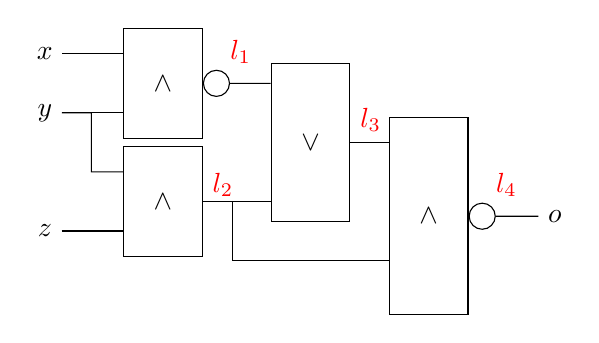
\begin{tikzpicture}
      \begin{scope}[scale=0.75]
        \node[rectangle,draw,minimum height=1.4cm,minimum width=1cm]
        (nand) at (2.5,3) {$\wedge$};
        \node[circle,draw,anchor=west,label={[red,xshift=-2]above right:$l_1$}] (nandneg) at (nand.east) {};
        \node[rectangle,draw,minimum height=1.4cm,minimum width=1cm,label={[red,yshift=6]right:$l_2$}]
        (andl) at (2.5,1) {$\wedge$};
        \node[rectangle,draw,minimum height=2cm,minimum width=1cm,label={[red,yshift=8]right:$l_3$}]
        (or) at (5,2) {$\vee$};
        \node[rectangle,draw,minimum height=2.5cm,minimum width=1cm]
        (andr) at (7,0.75) {$\wedge$};
        \node[circle,draw,anchor=west,label={[red,xshift=-2]above right:$l_4$}] (andneg) at (andr.east) {};
        \draw (nandneg.east) -- ($(or.north west)!(nand.east)!(or.south west)$);
        \draw (andl.east) -- ($(or.north west)!(andl.east)!(or.south west)$);
        \draw (or.east) -- ($(andr.north west)!(or.east)!(andr.south west)$);
        \node (inx) at (0.5,3.5) {$x$};
        \node (iny) at (0.5,2.5) {$y$};
        \node (inz) at (0.5,0.5) {$z$};
        \draw (inx.east) -- ($(nand.north west)!(inx.east)!(nand.south west)$);
        \draw (iny.east) -- ($(nand.north west)!(iny.east)!(nand.south west)$);
        \draw (inz.east) -- ($(nand.north west)!(inz.east)!(nand.south west)$);
        \draw (iny.east) -- ++(0.5,0) -- ++(0,-1) coordinate (tmp1) --
        ($(nand.north west)!(tmp1)!(nand.south west)$);
        \draw (andl.east) -- ++(0.5,0) -- ++(0,-1) coordinate (tmp2) --
        ($(andr.north west)!(tmp2)!(andr.south west)$);
        \node (out) at ($(andneg.east)+(1,0)$) {$o$};
        \draw (andneg.east) -- (out.west);
      \end{scope}
    \end{tikzpicture}
    \caption{Labeled circuit.}
    \label{fig:tseitin2}
  \end{figure}


  So the corresponding equivalences are (where $\uparrow$ is the Sheffer
  stroke for NAND gates):
  \begin{align*}
    l_1 &\leftrightarrow x \uparrow y\\
    l_2 &\leftrightarrow y \land z \\
    l_3 &\leftrightarrow l_1 \lor l_2 \\
    l_4 &\leftrightarrow l_3 \uparrow l_2\\
  \end{align*}

  Corresponding to those equivalences are the following clauses:
  \begin{align*}
    &\neg l_1 \lor \neg x \lor \neg y&& l_1 \lor x && l_1 \lor y\\
    &\neg l_2 \lor y && \neg l_2 \lor z&& l_2 \lor \neg y \lor \neg z\\
    &\neg l_3 \lor l_1 \lor l_2 && l_3 \lor \neg l_1 && l_3 \lor \neg l_2\\
    &\neg l_4 \lor \neg l_3 \lor \neg l_2 && l_1 \lor l_3 && l_1 \lor l_2
  \end{align*}

  We add the single clause $l_4$ to the above set and obtain a set of clauses
  corresponding to the above circuit, whose size is linear in the size of the
  circuit.
}

\end{enumerate}


\newpage

\Aufgabe[DLL Procedure and Implication Graphs \hfill \bf (1 point)]

\begin{enumerate}
\item Draw an implication graph starting with decisions $d=1@1$, $a=0@2$, apply BCP
  with clauses $c_1 = ( \neg d \lor b \lor a)$, $c_2 = (\neg b \lor c)$,
  $c_3=( \neg c \lor \neg d \lor \neg e)$, $c_4=( \neg e \lor \neg a)$,
  $c_5=( \neg b \lor \neg a \lor f)$, and $c_6=(\neg b \lor a \lor \neg g)$.

\solution{
  The resulting implication graph is given in Figure \ref{fig:ig}.


  \begin{figure}[h]
    \centering
    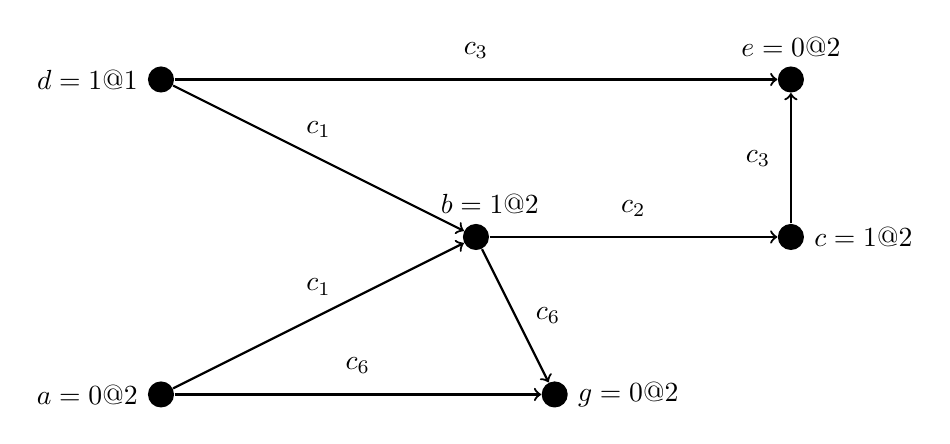
\begin{tikzpicture}
      \coordinate (d) at (-4,2);
      \coordinate (a) at (-4,-2);
      \coordinate (b) at (0,0);
      \coordinate (c) at (4,0);
      \coordinate (e) at (4,2);
      \coordinate (g) at (1,-2);
      
      \node[fill,circle,label=left:{$d=1@1$}] (dc) at (d) {};
      \node[fill,circle,label=left:{$a=0@2$}] (ac) at (a) {};
      
      \node[fill,circle,label=above:{$\quad b=1@2$}] (bc) at (b) {};
      \node[fill,circle,label=right:{$c=1@2$}] (cc) at (c) {};

      \draw[->,thick] (dc) --node[label=above:$c_1$] {} (bc);
      \draw[->,thick] (ac) --node[label=above:$c_1$] {} (bc);
      \draw[->,thick] (bc) --node[label=above:$c_2$] {} (cc);

      \node[fill,circle,label=above:{$e=0@2$}] (ec) at (e) {};
      \draw[->,thick] (dc) --node[label=above:$c_3$] {} (ec);
      \draw[->,thick] (cc) --node[label=left:$c_3$] {} (ec);

      \node[fill,circle,label=right:{$g=0@2$}] (gc) at (g) {};
      \draw[->,thick] (bc) --node[label=right:$c_6$] {} (gc);
      \draw[->,thick] (ac) --node[label=above:$c_6$] {} (gc);


    \end{tikzpicture}
    \caption{Implication Graph}
    \label{fig:ig}
  \end{figure}

}


\item Extract a satisfying assignment for the above clauses from the
  implication graph.

\solution{
  All clauses are satisfied by the above implication graph. Therefore any
  assignment with $a=0,b=1,c=1,d=1,e=0,$ and $f$ arbitrary, e.g., set $f=1$,
  satisfies the above clauses.
}

\end{enumerate}




\newpage

%%%%%%%%%%%%%%%%%%%%%%%%%%%%%%%%%%%%%%%%%%%%%%%%%%%%%%%%%%%%%%%%%%%%%%
\Aufgabe[First Order Logic \hfill \bf (1 point)]

Let $F$ be the formula $\forall x \exists y \big( P(x,y) \rightarrow P(x,x) \big)$.

\begin{enumerate}
\item Give a model $I_F$ for $F$. Show that $I_F$ is indeed a model of $F$.
\solution{

  We choose as universe $U = \{ 1,2 \}$ and as the interpretation function
  $I_F(P)=\{ (1,2), (1,1) \}$.

  Proof that $I_F \models F$ holds: 
  As $x$ is all-quantified, we consider both possible cases for the value of
  $x$.
  \begin{itemize}
  \item Case $x=1$: pick $y=2$, then $I_F(P(1,2))=1$ and $I_F(P(1,1))=1$, so
    the implication $P(1,2) \rightarrow P(1,1)$ holds, i.e., $I_F(P(1,2)
    \rightarrow P(1,1))=1$.
  \item Case $x=2$: pick $y=2$, then $I_F(P(2,2))=0$, therefore $I_F(P(2,2)
    \rightarrow P(2,2))=1$ as the antecedent is false.
  \end{itemize}


}

\item Is there an interpretation $I$ for $F$ which is no model of $F$?
  Either give such an $I$ or argue why none exists.

\solution{

  Claim: Every interpretation is a model of $F$ (i.e., $F$ is a tautology).

  For $F$ to be false, we need values for $x,y$ such that $P(x,y)$ holds while
  $P(x,x)$ must not hold.
  As $y$ is existentially quantified after $x$, we can always pick
  $y\mathop{:=}x$ and make the implication, and thus $F$, true.
}

\item Find a first-order formula $F'$, which is a contradiction
  (unsatisfiable). Prove that any interpretation $I'$ falsifies $F'$.
\solution{

  Let $F' = \neg F$, then $F'$ is unsatisfiable, as $F$ is a tautology.


}

\item 
Let $T$ be a theory consisting of the following formulas
\begin{align*}
  &\forall x,y,z \big( (x < y) \land (y < z) \rightarrow (x < z) \big), \text{ and}\\
  &\forall x,y \big( (x < y) \rightarrow \neg (y < x) \big).
\end{align*}
Let $\phi$ be the formula $\forall x,y \big( (x < y) \rightarrow \exists z ( x
< z \land z < y) \big)$.
\begin{enumerate}[(i)]
\item
  Which properties of the $<$-relation are described by $T$?

  \solution{
    Transitivity and a strong form of asymmetry
    (in particular $T$ requires antisymmetry and irreflexivity).
  }

\item
  Find a model of $T$ which also satisfies $\phi$.

  \solution{
    We pick
    $D_1 = \mathbb{Q}$, $I_1(<) = \{ \langle p, q \rangle \mid p, q \in \mathbb{Q},\ p < q \}$
    (i.e., the `usual' less-than relation over $\mathbb{Q}$).

    We have to prove that a) $I_1\models T$ and b) $I_1 \models \phi$.
    \begin{enumerate}[a)]
    \item Arbitrarily pick $a,b,c \in \mathbb{Q}$ such that $a<b$ and $b<c$.
      \begin{itemize}
      \item[Transitivity:] $I_1$ interprets $<$ as less-than relation,
        therefore $I_1(a<b)=1$ and $I_1(b<c)=1$. Furthermore $I_1(a<c)=1$ as
        $a<b<c$ and $a<c$ holds for $<$ on rational numbers.
        So $I_1((a<b) \land (b<c) \rightarrow (a<c))=1$.
      \item[Antisymmetry/Irreflexivity:] As $a<b$, we know that $b \not < a$,
        thus for $I_1$ this means that $I_1(a<b)=1$ and $I_1(b<a)=0$. So
        $I_1((a<b) \rightarrow \neg (b<a))=1$.
      \end{itemize}
      As $a,b,c$ were picked arbitrarily, above conclusions also hold for
      their universal closures, i.e., $I_1(\forall a,b,c ((a<b) \land
      (b<c) \rightarrow (a<c))=1$ and $I_1(\forall a,b (a<b) \rightarrow \neg
      (b<a))=1$. Now replacing $a,b,c$ with $x,y,z$ (respectively) shows that
      $I_1 \models T$.
    \item
      Arbitrarily pick $a,b \in \mathbb{Q}$ with $a<b$, we have to show that there exists
      a $c$ between $a$ and $b$. Let $c=a+(b-a)/2$, i.e., the rational number
      halfway between $a$ and $b$, which obviously exists.
      As $I_1$ interprets $<$ as usual less-than relation $I_1(a<b)=1$,
      $I_1(a<c)=1$, and $I_1(c<b)$ holds. So $I_1((a<b)\rightarrow \exists c(
      a<c \land c<b))=1$.

      As $a,b$ were picked arbitrarily, the same reasoning holds for the
      universal closure, i.e., for $\phi$ if $a,b,c$ is again replaced with
      $x,y,z$.
    \end{enumerate}
  }

\item
  Show that there is an interpretation which satisfies $T$ but does not
  satisfy $\phi$.

  \solution{
  $D_2 = \mathbb{N}$, $I_2(<) = \{ \langle p, q \rangle \mid p, q \in \mathbb{N},\ p < q \}$
  (i.e., the `usual' less-than relation over $\mathbb{N}$).

  Showing that $I_2 \models T$ is completely analogous to the previous
  exercise.

  It remains to show that $I_2 \not \models \phi$:
  Let $x=1,y=2$, then $I_2(x<y)=1$. As $I_2$ is defined over $\mathbb{N}$,
  there are no numbers between $1$ and $2$, i.e., $\not \exists z$ with
  $1<z \land z<2$. So $I_2(\exists z (1<z \land z<2) )=0$ and
  $I_2((1<2)\rightarrow \exists z( 1<z \land z<2))=0$.
 
  Therefore $I_2(\forall x,y (x<y)\rightarrow \exists z( x<z \land z<y))=0$
  and so $I_2 \not \models \phi$.
  }

\item 
  Check whether $\phi$ is $T$-satisfiable, and $T$-valid?

  \solution{
    \begin{itemize}
    \item As $I_1 \models T$ and $I_1 \models \phi$ it holds that $\phi$ is
      $T$-satisfiable.
    \item $T$-validity, however, does not hold as $I_2 \models T$, but $I_2
      \not \models \phi$.
    \end{itemize}
  }

\end{enumerate}

\end{enumerate}


\newpage

\Aufgabe[Problem Solving in FOL and PL0 \hfill \bf (1 point)]

4x4 Sudoku is a simplified form of Sudoku where only numbers $1, \ldots, 4$
occur and each quarter has 2x2 fields.


\begin{figure}[h!]
  \centering
  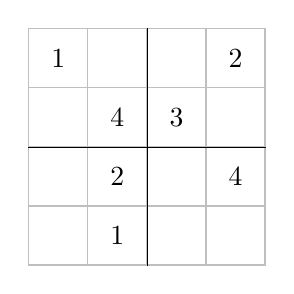
\begin{tikzpicture}
    \begin{scope}[scale=0.75]
      \begin{scope}[color=lightgray]
        % define fields
        \foreach \x in { 1, 2, 3, 4} {
          \foreach \y in { 1, 2, 3, 4} {
            \node[shape=rectangle,draw,minimum width=7.5mm,minimum height=7.5mm]
            (r\x \y) at (\x,6-\y) {};
          }
        }
      \end{scope}
      % grid
      \draw (r21.north east) -- (r24.south east);
      \draw (r12.south west) -- (r42.south east);

      % hints
      \node at (r11) {1};
      \node at (r22) {4};

      \node at (r41) {2};
      \node at (r32) {3};

      \node at (r23) {2};
      \node at (r24) {1};

      \node at (r43) {4};

    \end{scope}
  \end{tikzpicture}
\end{figure}

Let $p(r,c,n)$ encode that number $n$ is in row $r$ and column $c$.

\begin{enumerate}
\item Give a first order theory $T_S$ which encodes the solutions to such a
  4x4 Sudoko.

\solution{
  The following formulas ensure that any
  model of these formulas is a valid solution to our Sudoku instance.
  \begin{itemize}
  \item $T_{\mathit init}= p(1,1,1) \land p(2,2,4) \land p(2,3,3) \land p(1,4,2) \land p(3,2,2) \land
    p(4,2,1) \land p(3,4,4)$ \\ setting the initial numbers.
  \item $T_{\mathit dom} = \forall x : x=1 \lor x=2 \lor x=3 \lor x=4$ \\
    fix domain to $D_S=\{1,2,3,4\}$.
  \item $T_{\mathit val}= \forall r,c: \exists n: p(r,c,n)$ \\ assign a value to each cell.
  \item $T_{\mathit val'}= \forall r,c,n,n': \big( p(r,c,n) \land p(r,c,n')
    \big) \rightarrow n =n'$ \\ each cell is assigned at most one number.
  \item $T_{\mathit row} = \forall r,n: \exists c: p(r,c,n)$ \\ in each row
    occurs each number in some cell.
  \item $T_{\mathit col} = \forall c,n: \exists r: p(r,c,n)$ \\ in each column
    occurs each number in some cell.
  \item $T_{\mathit quarters} = \big\{ \forall n: p(o,o',n) \lor p(o+1,o',n) \lor
    p(o,o'+1,n) \lor p(o,o'+1,n) \mid o,o' \in \{1,3\} \big\}$ \\ each number occurs
    once in each quarter of the field.
  \end{itemize}
  $T_S = T_{\mathit quarters} \cup \{ T_{\mathit dom}, T_{\mathit init},
  T_{\mathit val}, T_{\mathit val'}, T_{\mathit row}, T_{\mathit col}\}$
  finally makes sure that each model of $T_S$ is solution to our Sudoku.

  Observe that by changing $T_{\mathit init}$ we can use the above formulas to
  solve other instances of 4x4 Sudoku.
}


\item Find an equivalent propositional theory $P_S$ encoding the same. You are
  free to use standard mathematical notation to state $P_S$ in shorter terms.

\solution{
  Using the formulas from $T_S$ above makes it easier to find a propositional
  theory $P_S$. Basically, all we have to do is getting rid of quantifiers.
  As a shorthand, let $D_S=\{1,2,3,4\}$ in the following.

  \begin{itemize}
  \item $P_{\mathit init} = T_{\mathit init}$ \\ as $T_{\mathit init}$ is
    already propositional.
  \item $P_{\mathit val} = \big\{ p(r,c,1) \lor p(r,c,2) \lor p(r,c,3) \lor
    p(r,c,4) \mid r,c \in D_S \big\}$ \\ enumerate all values for
    existentially-quantified variable $n$ and make a new formula for each
    combination of all-quantified variables $r,c$.
  \item $P_{\mathit val'} = \big\{ \neg\big( p(r,c,n) \land p(r,c,n') \big) \mid
    r,c,n,n' \in D_S  \land n \neq n' \big\}$ \\ ensure no cell is
    assigned two values.
  \item $P_{\mathit row} = \big\{ p(r,1,n) \lor \ldots \lor p(r,4,n) \mid r,n
    \in D_S \big\}$.
  \item $P_{\mathit col} = \big\{ p(1,c,n) \lor \ldots \lor p(4,c,n) \mid c,n
    \in D_S \big\}$.
  \item $P_{\mathit quarters} = \big\{ p(o,o',n) \lor p(o+1,o',n) \lor
    p(o,o'+1,n) \lor p(o,o'+1,n) \mid o,o' \in \{1,3\} \land n \in D_S \big\}$.
  \end{itemize}

  $P_S = \{ P_{\mathit init} \}  \cup  P_{\mathit val} \cup P_{\mathit val'}
  \cup P_{\mathit row} \cup P_{\mathit col} \cup P_{\mathit quarters}$ 
  then is a propositional encoding of the 4x4 Sudoku.
}

\item Transform $P_S$ into a set of clauses and give them to a SAT solver
  (e.g., MiniSat) to obtain the solution to the above sample Sudoku.

  State which solver you were using, give its input data (in whatever
  format it is) as well as the solver's output.

\solution{
  Excluded for space reasons.
}

\end{enumerate}

\newpage

%%%%%%%%%%%%%%%%%%%%%%%%%%%%%%%%%%%%%%%%%%%%%%%%%%%%%%%%%%%%%%%%%%%%%%%%%%%%%%
\Aufgabe[\hfill \bf (2 points)]

Let $\mathcal{C}$ be a clause set consisting of the following clauses:

\begin{eqnarray*}
  c_1 \colon &&( \neg A \lor B )\\
  c_2\colon &&( \neg A \lor \neg B \lor C )\\
  c_3\colon &&( A \lor B )\\
  c_4\colon &&( \neg F \lor \neg B \lor \neg G )\\
  c_5\colon &&( G \lor \neg E )\\
  c_6\colon &&( G \lor D )\\
  c_7\colon &&( C \lor E \lor \neg D )
\end{eqnarray*}

\begin{enumerate}[a)]
\item Draw an implication graph for $\mathcal{C}$. Use the decision $C=0@1$
  first and $A=1@2$ afterwards until you reach a conflict.

\solution{
  The resulting implication graph is given in Figure \ref{fig:ig1}.


  \begin{figure}[h]
    \centering
    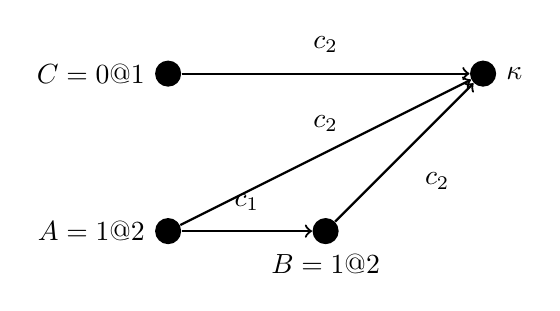
\begin{tikzpicture}
      \coordinate (c) at (0,0);
      \coordinate (a) at (0,-2);
      \coordinate (b) at (2,-2);
      \coordinate (k) at (4,0);
      
      \node[fill,circle,label=left:{$C=0@1$}] (cn) at (c) {};
      \node[fill,circle,label=left:{$A=1@2$}] (an) at (a) {};
      
      \node[fill,circle,label=below:{$B=1@2$}] (bn) at (b) {};
      \node[fill,circle,label=right:{$\kappa$}] (kn) at (k) {};

      \draw[->,thick] (an) --node[label=above:$c_1$] {} (bn);
      \draw[->,thick] (bn) --node[label=below right:$c_2$] {} (kn);
      \draw[->,thick] (cn) --node[label=above:$c_2$] {} (kn);
      \draw[->,thick] (an) --node[label=above:$c_2$] {} (kn);
    \end{tikzpicture}
    \caption{Implication Graph for $\mathcal{C}$ with $C=0@1$ and $A=1@2$.}
    \label{fig:ig1}
  \end{figure}
}


\item Determine a conflict clause, apply dependency-directed backtracking and
  continue the resulting implication graph with decision
  $F=1@3$ until you reach a conflict.

\solution{
  $c_8 \colon (\neg A \lor C)$ is a conflict clause, dependency-directed
  backtracking means we stay at $DL=2$, but erase the decision.
  We apply BCP to flip the value of $A$ using $c_8$.
  The resulting implication graph (before $F=1@3$) then is given in Figure
  \ref{fig:ig2}.

  \begin{figure}[h]
    \centering
    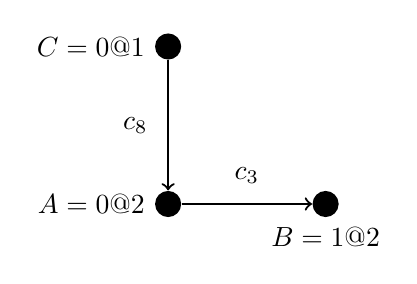
\begin{tikzpicture}
      \coordinate (c) at (0,0);
      \coordinate (a) at (0,-2);
      \coordinate (b) at (2,-2);
      
      \node[fill,circle,label=left:{$C=0@1$}] (cn) at (c) {};
      \node[fill,circle,label=left:{$A=0@2$}] (an) at (a) {};
      \node[fill,circle,label=below:{$B=1@2$}] (bn) at (b) {};

      
      \draw[->,thick] (cn) --node[label=left:$c_8$] {} (an);
      \draw[->,thick] (an) --node[label=above:$c_3$] {} (bn);
    \end{tikzpicture}
    \caption{Implication Graph for $\mathcal{C}$ with $C=0@1$ and $A=1@2$
      after learning $c_8 \colon (\neg A \lor C)$, dependency-directed
      backtracking, and BCP.}
    \label{fig:ig2}
  \end{figure}

  Setting $F=1@3$ and BCP results in the conflict graph of Figure \ref{fig:ig3}.

  \begin{figure}[h]
    \centering
    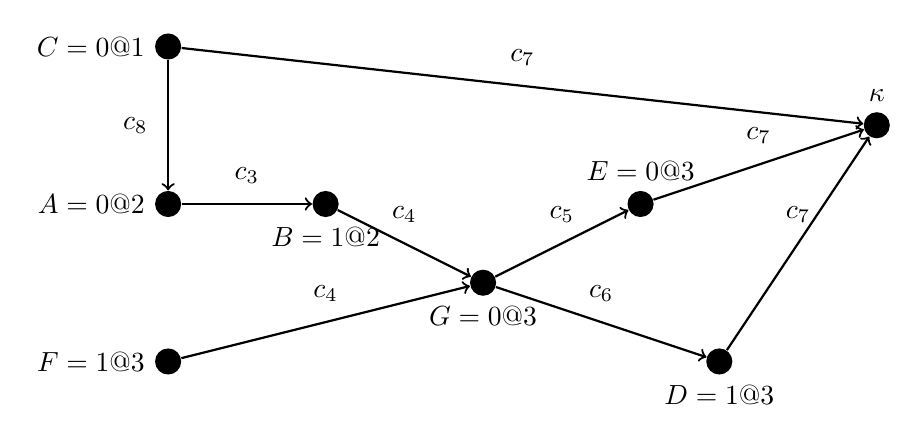
\begin{tikzpicture}
      \coordinate (c) at (0,0);
      \coordinate (a) at (0,-2);
      \coordinate (b) at (2,-2);
      \coordinate (f) at (0,-4);
      \coordinate (g) at (4,-3);
      \coordinate (e) at (6,-2);
      \coordinate (d) at (7,-4);
      \coordinate (k) at (9,-1);

      
      \node[fill,circle,label=left:{$C=0@1$}] (cn) at (c) {};
      \node[fill,circle,label=left:{$A=0@2$}] (an) at (a) {};
      \node[fill,circle,label=below:{$B=1@2$}] (bn) at (b) {};
      
      \draw[->,thick] (cn) --node[label=left:$c_8$] {} (an);
      \draw[->,thick] (an) --node[label=above:$c_3$] {} (bn);

      \node[fill,circle,label=left:{$F=1@3$}] (fn) at (f) {};
      \node[fill,circle,label=below:{$G=0@3$}] (gn) at (g) {};
      \node[fill,circle,label=below:{$D=1@3$}] (dn) at (d) {};
      \node[fill,circle,label=above:{$E=0@3$}] (en) at (e) {};

      \node[fill,circle,label=above:{$\kappa$}] (kn) at (k) {};


      \draw[->,thick] (bn) --node[label=above:$c_4$] {} (gn);
      \draw[->,thick] (fn) --node[label=above:$c_4$] {} (gn);
      \draw[->,thick] (gn) --node[label=above:$c_6$] {} (dn);
      \draw[->,thick] (gn) --node[label=above:$c_5$] {} (en);

      \draw[->,thick] (cn) --node[label=above:$c_7$] {} (kn);
      \draw[->,thick] (en) --node[label=above:$c_7$] {} (kn);
      \draw[->,thick] (dn) --node[label=above:$c_7$] {} (kn);
    \end{tikzpicture}
    \caption{Implication Graph for $\mathcal{C}$ with $C=0@1$ and $A=1@2$
      after learning $c_8 \colon (\neg A \lor C)$, dependency-directed
      backtracking, then decision $F=1@3$ and BCP.}
    \label{fig:ig2}
  \end{figure}

}

\item Determine all UIPs in the implication graph, find the first UIP and use
  resolution to learn a conflict clause corresponding to the first UIP.

\solution{
  UIPs (nodes through which all paths from the current decision to the
  conflict go through) are the nodes $F=1@3$ and $G=0@3$ where the latter is
  the first UIP (closest to the conflict).

  We resolve $c_7$, $c_5$, and $c_6$ and obtain:
  \begin{align*}
    r_1 := res(c_7,c_5,E) =& (C \lor G \lor \neg D)\\
    r_2 := res(r_1,c_6,D) =&( C \lor G \lor G)\\
    fac(r_2) = &( C \lor G )
  \end{align*}

  So the learned clause according to the first UIP scheme is $c_9 \colon (C
  \lor G)$.

}

\item Add the learned clause, apply conflict-driven backtracking and draw the
  resulting implication graph.

\solution{
  For conflict-driven backtracking, we backtrack to the second highest DL in
  the learned clause, i.e., we backtrack to $DL=1$. For this kind of
  backtracking, we keep all decisions on $DL=1$ but delete all others with
  $DL>1$. After BCP the resulting implication graph is as in Figure
  \ref{fig:ig3}.

  \begin{figure}[h]
    \centering
    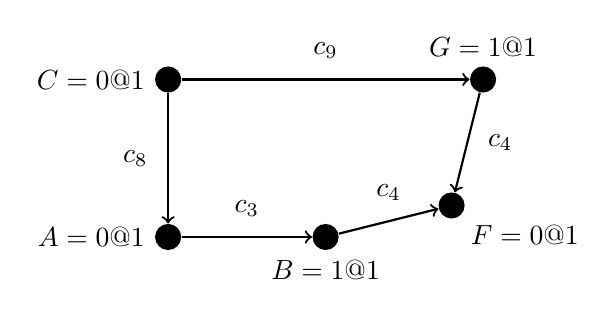
\begin{tikzpicture}
      \coordinate (c) at (0,0);
      \coordinate (a) at (0,-2);
      \coordinate (b) at (2,-2);
      \coordinate (f) at (3.6,-1.6);
      \coordinate (g) at (4,0);
      \coordinate (e) at (6,-2);
      \coordinate (d) at (7,-4);
      \coordinate (k) at (9,-1);

      
      \node[fill,circle,label=left:{$C=0@1$}] (cn) at (c) {};
      \node[fill,circle,label=left:{$A=0@1$}] (an) at (a) {};
      
      \node[fill,circle,label=above:{$G=1@1$}] (gn) at (g) {};
      \node[fill,circle,label=below:{$B=1@1$}] (bn) at (b) {};
      
      \draw[->,thick] (cn) --node[label=left:$c_8$] {} (an);
      \draw[->,thick] (cn) --node[label=above:$c_9$] {} (gn);
      \draw[->,thick] (an) --node[label=above:$c_3$] {} (bn);

      \node[fill,circle,label=below right:{$F=0@1$}] (fn) at (f) {};
      \draw[->,thick] (bn) --node[label=above:$c_4$] {} (fn);
      \draw[->,thick] (gn) --node[label=right:$c_4$] {} (fn);

    \end{tikzpicture}
    \caption{Implication Graph for $\mathcal{C}$ with learned clauses $c_8$
      and $c_9$ after conflict-driven backtracking and BCP.}
    \label{fig:ig3}
  \end{figure}


}
\item Consider the clause set $\mathcal{D}= \mathcal{C} \cup \{ (\neg A \lor
  C) \}$. State which would be the first variable assignment chosen by the
  DLIS decision heuristic for the clause set $\mathcal{D}$.

\solution{
  We have $C^+_C=3$ and $C^-_A=3$ (the values for all other variables are
  smaller), therefore DLIS would select $A=0@1$.
}

\end{enumerate}




\newpage

%%%%%%%%%%%%%%%%%%%%%%%%%%%%%%%%%%%%%%%%%%%%%%%%%%%%%%%%%%%%%%%%%%%%%%

\Aufgabe[Sparse Method \hfill \bf (2 points)]
For the following formula in equation logic apply the Sparse Method including
preprocessing (simplification) to compute an equisatisfiable formula in
propositional logic.
%
\def\eqs{\ensuremath{\,{=}\,}}
\def\neqs{\ensuremath{\,{\neq}\,}}
\begin{gather*}
  [ (x_1 \eqs x_2 \land x_1 \eqs x_3 ) \lor ( x_3 \eqs x_2 \land x_2 \eqs x_8)] \land \\
  x_2 \neqs x_4 \land 
  ( x_8 \eqs x_4 \lor x_8 \neqs x_7 ) \land \\
  ( x_5 \eqs x_4 \lor x_5 \neqs x_7 ) \land 
  ( x_6 \eqs x_7 \lor x_6 \eqs x_5)
\end{gather*}

\solution{

  Let $\varphi^E$ be the above formula, then the equality graph $G^E(\varphi^E)$ is
  given in Figure \ref{fig:sp1}. Dashed lines represent equality edges while
  solid lines represent disequality edges.

  \begin{figure}[h]
    \centering
    \begin{tikzpicture}
      \node(x1){$x_1$};
      \node[right=of x1](x2){$x_3$};
      \node[right=of x2](x3){$x_2$};
      \node[below=of x3](x4){$x_4$};
      \node[left=of x4](x5){$x_8$};
      \node[below=of x5](x6){$x_7$};
      \node[right=of x6](x7){$x_5$};
      \node at($(x7)+(-.8cm,-1.2cm)$)(x8){$x_6$};
      
      \draw[dashed] (x1) -- (x2);
      \draw[dashed] (x2) -- (x3);
      \draw[dashed] (x1.north) parabola[parabola height=1cm] (x3.north);
      
      \draw[dashed] (x3) -- (x5);
      \draw[] (x3) -- (x4);
      \draw[dashed] (x4) -- (x5);
      \draw[] (x5) -- (x6);
      \draw[dashed] (x4) -- (x7);
      \draw[] (x6) -- (x7);
      \draw[dashed] (x6) -- (x8);
      \draw[dashed] (x7) -- (x8);
    \end{tikzpicture}
    \caption{$G^E(\varphi^E)$, dashed lines represent equality, solid lines disequality.}
    \label{fig:sp1}
  \end{figure}

  Edges $(x_1,x_2), (x_2,x_3)$, and $(x_1,x_3)$ are not part of a simple
  contradictory cycle, therefore we set those edges to $true$ in $\varphi^E$
  and obtain $\varphi^E_2$ as:
  
  \begin{gather*}
    [ (true \land true ) \lor ( true \land x_2 \eqs x_8)] \land \\
    x_2 \neqs x_4 \land 
    ( x_8 \eqs x_4 \lor x_8 \neqs x_7 ) \land \\
    ( x_5 \eqs x_4 \lor x_5 \neqs x_7 ) \land 
    ( x_6 \eqs x_7 \lor x_6 \eqs x_5)
  \end{gather*}

  Propositional simplification of $\varphi^E_2$ leads to $\varphi^E_3$ as:
  \begin{gather*}
    x_2 \neqs x_4 \land 
    ( x_8 \eqs x_4 \lor x_8 \neqs x_7 ) \land \\
    ( x_5 \eqs x_4 \lor x_5 \neqs x_7 ) \land 
    ( x_6 \eqs x_7 \lor x_6 \eqs x_5)
  \end{gather*}

  We draw the equality graph $G^E(\varphi^E_3)$, given in Figure \ref{fig:sp2}.

  \begin{figure}[h]
    \centering
    \begin{tikzpicture}
      \node(x1){};
      \node[right=of x1](x2){};
      \node[right=of x2](x3){$x_2$};
      \node[below=of x3](x4){$x_4$};
      \node[left=of x4](x5){$x_8$};
      \node[below=of x5](x6){$x_7$};
      \node[right=of x6](x7){$x_5$};
      \node at($(x7)+(-.8cm,-1.2cm)$)(x8){$x_6$};
      
      \draw[] (x3) -- (x4);
      \draw[dashed] (x4) -- (x5);
      \draw[] (x5) -- (x6);
      \draw[dashed] (x4) -- (x7);
      \draw[] (x6) -- (x7);
      \draw[dashed] (x6) -- (x8);
      \draw[dashed] (x7) -- (x8);
    \end{tikzpicture}
    \caption{$G^E(\varphi^E_3)$, dashed lines represent equality, solid lines disequality.}
    \label{fig:sp2}
  \end{figure}

  Now $x_2 \neqs x_4$ is not contained in any simple contradictory cycle and
  we set it to $true$ and apply propositional simplification. The result is
  $\varphi^E_4$ as:

  \begin{gather*}
    ( x_8 \eqs x_4 \lor x_8 \neqs x_7 ) \land \\
    ( x_5 \eqs x_4 \lor x_5 \neqs x_7 ) \land 
    ( x_6 \eqs x_7 \lor x_6 \eqs x_5)
  \end{gather*}



  As there are no more literals not occurring in a simple contradictory cycle,
  we stop preprocessing and build the propositional skeleton $e(\varphi^E_4)$ by
  replacing equality literals $x_i \eqs x_j$ with $e_{i,j}$, so
  \begin{gather*}
    e(\varphi^E_4) = (e_{4,8} \lor \neg e_{7,8}) \land 
    (e_{4,5} \lor e_{5,7}) \land
    (e_{6,7} \lor e_{5,6})
  \end{gather*}

  To derive a (small) set of transitivity constraints ($B_t$), we take the nonpolar
  equality graph $G^E_{NP}(\varphi^E_4)$ and make it chordal. $G^E_{NP}$ is
  given in Figure \ref{fig:sp3}

  \begin{figure}[h]
    \centering
    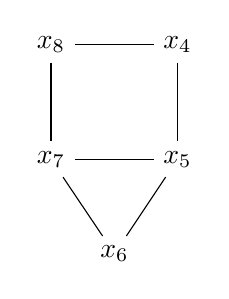
\begin{tikzpicture}
      \node[](x4){$x_4$};
      \node[left=of x4](x5){$x_8$};
      \node[below=of x5](x6){$x_7$};
      \node[right=of x6](x7){$x_5$};
      \node at($(x7)+(-.8cm,-1.2cm)$)(x8){$x_6$};
      %
      \draw[] (x4) -- (x5);
      \draw[] (x5) -- (x6);
      \draw[] (x4) -- (x7);
      \draw[] (x6) -- (x7);
      \draw[] (x6) -- (x8);
      \draw[] (x7) -- (x8);
    \end{tikzpicture}
    \caption{$G^E_{NP}$}
    \label{fig:sp3}
  \end{figure}
  
  To make it chordal, we have two alternatives, i.e., either to add
  $(x_5,x_8)$ or to add $(x_4,x_7)$. We add the edge $(x_5,x_8)$. This leads
  to a graph where no simple cycle has length greater than $3$, i.e., the
  graph in Figure \ref{fig:sp4} is ``triangular'' and thus chordal.
  
  \begin{figure}[h]
    \centering
    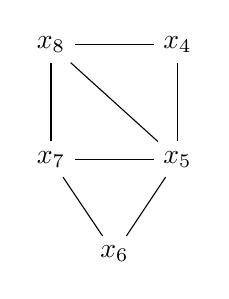
\begin{tikzpicture}
      \node[](x4){$x_4$};
      \node[left=of x4](x5){$x_8$};  % 5 -- 8
      \node[below=of x5](x6){$x_7$}; % 6 --7
      \node[right=of x6](x7){$x_5$}; % 7 -- 5
      \node at($(x7)+(-.8cm,-1.2cm)$)(x8){$x_6$}; % 8 -- 6
      
      \draw[] (x4) -- (x5);
      \draw[] (x5) -- (x6);
      \draw[] (x4) -- (x7);
      \draw[] (x6) -- (x7);
      \draw[] (x6) -- (x8);
      \draw[] (x7) -- (x8);
      \draw[] (x5) -- (x7);
    \end{tikzpicture}
    
    \caption{$G^E_{NP}$ made chordal by adding edge $(x_8,x_5)$.}
    \label{fig:sp4}
  \end{figure}

  For each triangle in this graph, we derive the according transitivity
  constraints to obtain $B_t$.
  \begin{eqnarray*}
    B_t:= &(e_{4,8} \land e_{5,8} \rightarrow e_{4,5}) \land
    (e_{5,8} \land e_{4,5} \rightarrow e_{4,8}) \land
    (e_{4,5} \land e_{4,8} \rightarrow e_{5,8}) \land & \quad \quad \text{for }\triangle
    (x_4,x_8,x_5)\\
    %
    &(e_{6,7} \land e_{5,7} \rightarrow e_{5,6}) \land
    (e_{5,7} \land e_{5,6} \rightarrow e_{6,7}) \land
    (e_{5,6} \land e_{6,7} \rightarrow e_{5,7}) \land & \quad \quad \text{for
    } \triangle (x_6,x_7,x_5)\\
    %
    &(e_{5,7} \land e_{5,8} \rightarrow e_{7,8}) \land
    (e_{5,8} \land e_{7,8} \rightarrow e_{5,7}) \land
    (e_{7,8} \land e_{5,7} \rightarrow e_{5,8}) &\quad \quad\text{for }  \triangle (x_7,x_5,x_8)
  \end{eqnarray*}

  The final formula then is $e(\varphi^E_4) \land B_t$.

}



\newpage


%%%%%%%%%%%%%%%%%%%%%%%%%%%%%%%%%%%%%%%%%%%%%%%%%%%%%%%%%%%%%%%%%%%%%%%%%%%%%%

\Aufgabe[Ackermann's and Bryant's Reductions \hfill \bf (2 points)]
Reduce the problem of validity of the following EUF-formula
\begin{gather*}
  F(F(x_1)) \neq F(x_1) \land G(x_1,x_2) = F(x_2) \land F(G(x_2,F(x_2))) \neq F(F(x_1))
\end{gather*}
to the problem of validity in equation logic
\begin{enumerate}[a)]
\item using Ackermann's reduction.

\solution{
  We first number the instances of the UFs inwards-to-outwards, left-to-right:
  \begin{gather*}
    F_2(F_1(x_1)) \neq F_1(x_1) \land G_1(x_1,x_2) = F_3(x_2) \land F_4(G_2(x_2,F_3(x_2))) \neq F_2(F_1(x_1))
  \end{gather*}
  
  This already gives $\cT$ for the numbered instances. For example:
  \begin{align*}
    \cT (F_1(x_1)) &= f_1\\
    \cT (F_2(F_1(x_1))) &= f_2\\
    \cT (F_3(x_2)) &= f_3 \\
    \cT (F_4(G_2(x_2,F_3(x_2)))) &= f_4 \\
    \cT (G_1(x_1,x_2)) &= g_1\\
    \cT (G_2(x_2,F_3(x_2))) &= g_2
  \end{align*}


  So $flat^E:= f_2 \neq f_1 \land g_1 = f_3 \land f_4 \neq f_2$.

  Based on $\cT$ we construct $FC^E :=$
  \def\impl{\rightarrow}
  \begin{align*}
    (x_1 = f_1 \impl& f_1 = f_2) \land \\
    (x_1 = x_2 \impl& f_1 = f_3) \land \\
    (x_1 = g_2 \impl& f_1 = f_4) \land \\
    (f_1 = x_2 \impl& f_2 = f_3) \land \\
    (f_1 = g_2 \impl& f_2 = f_4) \land \\
    (x_2 = g_2 \impl& f_3 = f_4) \land \\
    (( x_1 = x_2 \land x_2 = f_3 ) \impl& g_1 = g_2)
  \end{align*}

  Finally $\varphi^E := FC^E \impl flat^E$.
}

\item using Bryant's reduction.

\solution{

  We re-use the numbering of function instances from the previous exercise and
  directly get $flat^E$ but each $F_i$ is now replaced with $F_i^*$ instead of
  $f_i$.

  So $flat^E:= F_2^* \neq F_1^* \land G_1^* = F_3^* \land F_4^* \neq F_2^*$.

  Each $F_i/G_i$ is first translated into a case-statement and then to a
  disjunctive formula to obtain $FC^E$.

\def\true{\mathit{true}}

  \begin{align*}
    F_1^* =&
    \left(\begin{array}{lr@{ \colon }l}
      \mathit{case} & \true & f_1
    \end{array}\right)\\
    F_2^* =&
    \left(\begin{array}{lr@{ \colon }l}
      \mathit{case} & x_1=F^*_1 & f_1 \\
      & \true & f_2
    \end{array}\right)\\
    F_3^* =&
    \left(\begin{array}{lr@{ \colon }l}
      \mathit{case} & x_1=x_2 & f_1 \\
      & F^*_1=x_2 & f_2 \\
      & \true & f_3
    \end{array}\right)\\
    F_4^* =&
    \left(\begin{array}{lr@{ \colon }l}
      \mathit{case} & x_1=G^*_2 & f_1 \\
      & F^*_1=G^*_2 & f_2 \\
      & x_2 =G^*_2 & f_3 \\
      & \true & f_4
    \end{array}\right)\\
    G_1^* =&
    \left(\begin{array}{lr@{ \colon }l}
      \mathit{case} & \true & g_1 \\
    \end{array}\right)\\
    G_2^* =&
    \left(\begin{array}{lr@{ \colon }l}
      \mathit{case} & x_1=x_2 \land x_2=F^*_3 & g_1 \\
      & \true &  g_2
    \end{array}\right)\\
  \end{align*}

  Each of those matrices has to be translated to an equality logic formula:

  
  \hspace{-4.6em}
  \begin{minipage}{1.0\linewidth}
  \begin{align*}
    F_1^* =&
    \left(\begin{array}{lr@{ \colon }l}
      \mathit{case} & \true & f_1
    \end{array}\right) & = &
    \begin{array}{lr}
        F_1^*=f_1 \land \true
    \end{array} &=: C(F^*_1)\\
    F_2^* =&
    \left(\begin{array}{lr@{ \colon }l}
      \mathit{case} & x_1=F^*_1 & f_1 \\
      & \true & f_2
    \end{array}\right) & = &
    \left(\begin{array}{lr}
      F_2^*=f_1 \land x_1=F^*_1& \lor\\
      F_2^*=f_2 \land \true \land x_1 \neq F^*_1
    \end{array}\right) &=: C(F^*_2)\\
    F_3^* =&
    \left(\begin{array}{lr@{ \colon }l}
      \mathit{case} & x_1=x_2 & f_1 \\
      & F^*_1=x_2 & f_2 \\
      & \true & f_3
    \end{array}\right) & = &
    \left(\begin{array}{lr}
      F_3^*=f_1 \land x_1=x_2& \lor\\
      F_3^*=f_2 \land F^*_1=x_2 \land x_1 \neq x_2 & \lor\\
      F_3^*=f_3 \land \true \land F^*_1 \neq x_1 \land x_1 \neq x_2 
    \end{array}\right) &=: C(F^*_3)\\
    F_4^* =&
    \left(\begin{array}{lr@{ \colon }l}
      \mathit{case} & x_1=G^*_2 & f_1 \\
      & F^*_1=G^*_2 & f_2 \\
      & x_2 =G^*_2 & f_3 \\
      & \true & f_4
    \end{array}\right) & = &
    \left(\begin{array}{lr}
      F_4^*=f_1 \land x_1=G^*_2& \lor\\
      F_4^*=f_2 \land F^*_1 =G^*_2 \land x_1 \neq G^*_2 & \lor\\
      F_4^*=f_3 \land x_2= G^*_2 \land F^*_1 \neq G^*_2 \land x_1 \neq G^*_2 & \lor\\
      F_4^*=f_4 \land \true \land x_2 \neq G^*_2 \land F^*_1 \neq G^*_2 \land x_1 \neq G^*_2
    \end{array}\right) &=: C(F^*_4) \\
    G_1^* =&
    \left(\begin{array}{lr@{ \colon }l}
      \mathit{case} & \true & g_1 \\
    \end{array}\right) & = &
    \left(\begin{array}{lr}
      G_1^*=g_1\\
    \end{array}\right) &=: C(G^*_1)\\
    G_2^* =&
    \left(\begin{array}{l@{\,}r@{ \colon }l}
      \mathit{case} & x_1{=}x_2 \land x_2{=}F^*_3 & g_1 \\
      & \true &  g_2
    \end{array}\right) \hspace*{-1em}& = &
    \left(\begin{array}{lr}
      G_2^*=g_1 \land x_1=x_2 \land x_2=F^*_3& \lor\\
      G_2^*=g_2 \land \true \land \neg(x_1 = x_2 \land x_2=F^*_3)
    \end{array}\right) &=: C(G^*_1)\\
  \end{align*}
  \end{minipage}


  Then $\varphi^E:= \left( \bigwedge_{1 \leq i \leq 4} C(F^*_i) 
    \bigwedge_{1 \leq i \leq 2} C(G^*_i) \right) \impl flat^E$.

}

\end{enumerate}

(Hint: The algorithms can be found on p.~67 and p.~70 
in D.~Kroening, O.~Strichman. Decision Procedures, Springer, 2008.
You find scans of the relevant chapter in the folder with background
material on Tuwel.)




\end{document}
